\documentclass[a4paper]{article}
\usepackage{amsmath,amsfonts,amsthm}
\usepackage{fullpage}
\usepackage{float}
\usepackage{color}
\usepackage{graphicx}
\usepackage{subfig}
\usepackage{authblk}
\usepackage{tikz-qtree}
\usepackage{float}
\title{Multiscale Adaptive Representation of Signals}
\author[1]{Cheng Tai}
\author[2]{Weinan E}
\affil[1]{PACM, Princeton University}
\affil[2]{Department of Mathematics and PACM, Princeton University}
\begin{document}

\newtheorem{lem}{Lemma}
\newtheorem{prop}{Proposition}
\newtheorem{rem}{Remark}
\newtheorem{thm}{Theorem}
\renewcommand{\a}{\mathbf{a}}
\renewcommand{\v}{\mathbf{v}}

\date{}
\maketitle
\abstract{In this paper, we present a model that gives rise to a multi-scale adaptive representation of image signals. This representation improves over dictionary learning in two ways: first, the encoding efficiency is dramatically improved; second, it is truly multi-scale. The proposed model is constructed by stacking several layers of units and each unit is an adaptive wavelet tight frame. Numerical illustrations are also given to show the effectiveness of this new representation.}

\section{Overview of Dictionary Learning and Wavelet Tight Frames}
It is now well acknowledged that sparse and overcomplete representations of data play a key role in many signal processing applications. The ability to represent a signal as a sparse linear combination of a few atoms from a possibly overcomplete dictionary lies in the heart of many applications including image/audio compression, denoising, and higher level tasks such as pattern recognition.

Over the years, many efforts have been put on designing dictionaries with certain properties. There are two main approaches towards this objective.  One approach can be loosely called the analytic dictionary approach, which assumes the mathematical properties of the class of signals of interest, and develops optimal representations for that class of signals. Examples in this category include: Fourier basis, wavelets, wavelet tight frames\cite{daubechies2003framelets}, curvelets\cite{candes2000curvelets}, contourlets\cite{do2002contourlets}, etc. The other approach takes a different route, it does not make any assumptions about the mathematical properties of the signals, instead it tries to learn the optimal dictionaries directly the data that give rise to sparse representations. More specifically, given the data matrix $X$, ones finds the dictionary $D$ and coefficients $C$ simultaneously by solving:
\begin{equation}
	\min_{D,C} \|X-DC\|_2^2 +\lambda \|C\|_1.
\end{equation}
Different dictionary learning models differ in the way the dictionary $D$ is updated. Examples of in category include: MOD\cite{engan1999method}, K-SVD\cite{aharon2006svd} and their variants, etc. Since the seminal work of Olshausen and Field\cite{olshausen1996emergence}, the field of dictionary learning has seen many promising advances.

The different nature of the two approaches result in different implementation schemes. Models of the first kind are characterized by implicit transformations whereas models of the second kind often explicitly apply the learned dictionary. The major advantage of the dictionary learning approach is that it leads to state-of-the art results in many low level signal processing applications. 

Despite the elegance and success of dictionary learning methodology, there are some shortcomings that cannot be ignored especially when the models are plugged into applications, these include the following:
\begin{itemize}
\item computational cost is high. Assume the signal is of length $N$, the trained dictionary $A\in \mathbb{R}^{m\times N}$ is stored and used explicitly. Each multiplication of the form $Ax$ requires $O(mN)$ operations. When dictionary learning models are learned and ready to use, we have to solve a sparse coding program, even with the fast greedy algorithms, such as Matching Pursuit, the matrix multiplications still have to be carried out several times. In comparison, the analytic dictionaries are much more efficient. The fast Fourier transform, takes $O(N\log N)$ operations and the one level wavelet transform takes only $O(N)$ operations. Hence the current dictionary learning approach is much less efficient compared to traditional transform methods.
\item restriction to low-dimensions. Because the learning procedure requires solving a relative complex non-convex optimization program, the signals that can be practically trained is restricted to have low dimensions, typically, $n\leq 1000$ is a reasonable limit. Partially because of this, in image processing applications, most popular models only train dictionaries on small image patches. An attempt to go beyond the size limit raises a series of problems, including the need for an huge amount of training data and intolerable training time.
\item operating on a single scale. Dictionaries as obtained by the MOD and the K-SVD operate at a single small scale. This issue is actually related to the previous ones, since the dictionary atoms that can be trained is small in size, which does not allow much room for multiple scales.  But past experience with wavelets has taught us that often times it is beneficial to process the signals at several scales, and operates on each scale separately. There are some attempts in training multi-scale dictionaries, this direction has yet to be thoroughly explored.
\item Artifacts.  In low level tasks such as image compression, the dictionary learning approach operates in a patch by patch manner, which produces visually unpleasant block effects along the boarders of the patch,\cite{bryt2008compression}.  Post processing is often needed to remove these artifacts\cite{bryt2008improving}. 
\end{itemize}

Given the good performance of dictionary learning and their shortcomings compared with traditional transforms, a natural question is, is there any hope to get the best of both worlds? It is the goal of this paper to propose a partial solution to this question. In particular, we address two issues: the inefficiency of sparse coding used by most dictionary learning scheme to encode a new signal and the lack of a truly multi-scale representation. We will devise a novel representation of image signals, which is multi-scale in nature and is computationally efficient, and it is adapted to the signals as dictionary learning does. 

In particular, we propose a model consists of several units stacked on top of each other, and each unit is itself an adaptive wavelet tight frame. The wavelet tight frames are constructed in a manner that gives the sparest representations of the signals within all the admissible tight frames.

\section{One Layer Adaptive Wavelet Tight Frames}

\subsection{Wavelet Tight Frames}
In this subsection, we give a very brief introduction to wavelet tight frames which the proposed model will be based upon. For a detailed introduction to this subject, the readers may refer to \cite{shen2010wavelet,daubechies2003framelets}.

Let $\mathcal{H}$ be a Hilbert space, we are mainly concerned with the case when $\mathcal{H}=L_p(\mathbb{R}^d)$. a system $X\subset \mathcal{H}$ is called a tight frame if
\[
\|f\|_2^2 = \sum_{x\in X} |\langle f,x\rangle |^2, \quad \textrm{for any } f\in \mathcal{H}
\]
There are two operators that are associated with a tight frame, one is the analysis operator defined as
\[
W: f\in \mathcal{H} \rightarrow \{\langle x,f\rangle\}_{x\in X} \in l_2(\mathbb{N})
\]
and the other is the synthesis operator $W^T$, which is the adjoint operator of the analysis operator defined as
\[
W^T : \{a_n\} \in l_2(\mathbb{N}) \rightarrow \sum_{x\in X} a_n x\in \mathcal{H}.
\]
The system $X$ is a tight frame if and only if $W^TW=I$, where $I: \mathcal{H} \rightarrow \mathcal{H}$ is the identity operator. In other words, given a tight frame $X$, we have the following canonical expansion:
\[
f=\sum_{x\in X} \langle x,f\rangle x, \quad \textrm{for any } f\in \mathcal{H}
\]
The sequence $Wf:=\{\langle f,x\rangle \}_{x\in X}$ are called the canonical tight frame coefficients. Thus, tight frames are often viewed as generalizations of orthonormal basis. In fact, a tight frame $X$ is an orthonormal basis for $\mathcal{H}$ if and only if $\|x\|=1,\forall x\in X$.

In signal processing applications, one widely used class of tight frames is the wavelet tight frames. The construction starts with a finite set of generators $\Psi:=\{\psi^1,\cdots,\psi^m\}$. Then consider the affine system defined by the shifts and dilations of the generators:
\[
X(\Psi)=\{M^{j/2}\psi^{l}(M^j\cdot -k),1\leq l\leq m, j,k\in\mathbb{Z}, M\in\mathbb{Z^+}\}.
\]
The affine system $X(\Psi)$ is called a wavelet tight frame if it is a tight frame satisfying
\[
f=\sum_{x\in X(\Psi)} \langle f,x\rangle x, \forall f \in \mathcal{H}.
\]
Wavelet tight frames used in practice are usually constructed from multi-resolution analysis(MRA). This is because a MRA structure enables fast decomposition and reconstruction algorithms.  The MRA construction usually starts with a compactly supported scaling function $\phi$ with a refinement mask  $a_0$ satisfying
\[
\hat{\phi}(M\cdot)=\hat{a_0}\hat{\phi}.
\]
where $\hat{\phi}$ is the Fourier transform of $\phi$, and $\hat{a_0}$ is the discrete Fourier series defined as
\begin{equation}
 \hat{a_0}(\omega):=\sum_{k\in\mathbb{Z}} a_0(k) e^{-ik\omega} \quad \textrm{and }\quad \hat{a_0}(0)=1.
\end{equation}
 After obtaining the scaling function, the next step step is to find an appropriate set of filters $\{a_1,\cdots,a_m\}$ and define the set of functions called framelets $\Psi=\{\psi_1,\cdots,\psi_m\}$ by
\[
\hat{\psi_i}(M\cdot) = \hat{a_i}\hat{\phi},i=1,\cdots,m
\]
such that the affine system $X(\Psi)$ forms a wavelet tight frame. 

Given the filters $\{a\}_{i=0}^m \in l_2(\mathbb{Z})$, the discrete decomposition and reconstruction transform are defined in the following way. Define the one dimensional down-sampling and up-sampling operator:
\[
\begin{aligned}
	&[v\downarrow M](n):=v(Mn),\quad n\in \mathbb{Z}\\
	&[v\uparrow](Mn):=v(n), \quad n\in \mathbb{Z}
\end{aligned}
\]
where $M$ a positive integer denoting the down-sampling or up-sampling factor.

Define the linear convolution operator $S_a: l_2(\mathbb{Z}) \rightarrow l_2(\mathbb{Z})$ by 
\[
[S_a(v](n):=[a*v](n)=\sum_{k\in\mathbb{Z}} (a(-\cdot)*v \downarrow)M, \forall v\in l_2(\mathbb{Z})
\]
For a set of filters $\{a_i\}_{i=1}^m\subset l_2(\mathbb{Z})$, we define its analysis operator $W$ by 
\[
W=[S_{a_1(-\cdot)},S_{a_2(-\cdot)},\cdots,S_{a_m(-\cdot)}]^T.
\]
Its synthesis operator is defined as the transpose of $W$:
\[
W^T=[S_{a_1(\cdot)},S_{a_2(\cdot)},\cdots, S_{a_m(\cdot )}].
\]
Note that $W$ and $W^T$ are in general very huge matrix, this notation merely indicates that they are linear operators and in practical, we always use convolution instead of using explicit matrix multiplication. We also use the notation $W_a$ and $W^T_a$ to indicate the dependence on the filters $\{a\}_{i=0}^m$.
It is natural to ask when the wavelet system $\Psi(X)$ forms a wavelet tight frame. Sufficient and necessary conditions are given by the so called Unitary Extension Principle(UEP). There are several versions of the unitary extension principles, in particular, we are interested in the one that is associated with discrete wavelet tight frames. For a survey of UEP, the reader may refer to \cite{benedetto2001wavelet}. The unitary extension principle states that:
\begin{thm}\cite{han2011adaptive}
Let $a_1,\cdots,a_m$ be finitely supported filters, the following are equivalent:
\begin{enumerate}
\item $W_a^T W_a = I$
\item for all $\omega \in [0,1)^d\cup M^{-1}\mathbb{Z}^d$,
\[
	\sum_{i=1}^m \hat{a_i}\overline{\hat{a_i}(\xi + 2\pi\omega})=\delta(\omega);
\]
\item for  all $k,\gamma \in \mathbb{Z}^d$,
\[
	\sum_{i=1}^m \sum_{n\in\mathbb{Z}^d} \overline{a_i(k+Mn+\gamma)}a_i(Mn+\gamma)=M^{-d}\delta(k).
\]
\end{enumerate}
\end{thm}
In particular, if the data are real numbers and no down-sampling is performed, then $W^TW=I$ is equivalent to 
\begin{equation}
\label{eq:uep}
\sum_{i=1}^m \sum_{n\in \mathbb{Z}^d} a_i(k+n) a_i(n)=\delta_k, \forall k\in \mathbb{Z}^d.
\end{equation}
We call all these conditions the UEP conditions. The linear B-spline wavelet tight frame used in many image restoration tasks is constructed via the UEP. Its associated tree filters are :
\[
a_1=\frac{1}{4}(1,2,1)^T; \quad a_2=\frac{\sqrt{2}}{4}(1,0,-1)^T; \quad a_3=\frac{1}{4}(-1,2,-1)^T.
\]
Once the 1D filter $\{a_i\}_{i=1}^m$ for generating a tight frame for $l_2(\mathbb{Z})$ is constructed, the traditional way of generating higher dimensional tight frames is to use tensor products of 1D filters.

\subsection{Adaptive Construction}
The aforementioned wavelet tight frame is a shift-invariant system. We use shift-invariant systems because we accept the premise that at some proper scales, the statistical properties of image patches are translational invariant. Let $W_a$ and $W_a^T$ be defined as before. Define $\mathcal{C}$ to be the set of filters that satisfy the full UEP condition, that is $\mathcal{C}=\{ \{a_i\}_{i=1}^m : W_a^TW_a=I\}$. In some image processing applications, a small loss of information is acceptable, we also consider the set of filters that approximately satisfy the full UEP condition within error $\delta$, $\mathcal{C}_\delta = \{\{a_i\}_{i=1}^m : \|W_a^TW_a -I\|_*\leq \delta\}$, where $\| \cdot \|_*$ means the operator norm.

For a specific class of images at hand, there are infinitely many discrete wavelet tight frames to choose from. Although they all provide perfect reconstruction of the input signal, some of them may provide sparser representations than the rest. It is natural to seek the filters that provide the sparest representation. That is, we look for the minimizer of the following optimization program:
\begin{equation}
\begin{aligned}
	&\min_{a_1,\cdots,a_m} \sum_{i=1}^m\Phi(v_i)\\
	\textrm{subject to} \quad &v_i = a_i(-\cdot)*x,\quad i=1,\cdots,m\\
	  &\{a_i\}_{i=1}^m \in \mathcal{C} \\
\end{aligned}
\end{equation}
where $\Phi(v_i)$ is a sparsity inducing function, it can be chosen as, for example, the $l_1$ norm or $l_0$ "norm" or the Huber loss. In our experiments, using different sparsity inducing terms does not seem to have much influence on the results, $l_1$ norm is slightly better in image restoration tasks. Hence we use $l_1$ norm in the following exclusively, this leads to:

\begin{equation}
\label{model:m0}
\begin{aligned}
	&\min_{a_1,\cdots,a_m} \sum_{i=1}^m \|v_i\|_1 \\
	\textrm{subject to} \quad&v_i = a_i(-\cdot)*x,\quad i=1,\cdots,m\\
	 & \{a_i\}_{i=1}^m \in \mathcal{C} \\
\end{aligned}
\end{equation}
In some higher level image processing tasks, such as pattern recognition, a small deviation from the perfect reconstruction filters is acceptable. In that case, we consider
\begin{equation}
\label{model:m1}
\begin{aligned}
	&\min_{a_1,\cdots,a_m} \sum_{i=1}^m \|v_i\|_1 \\
	\textrm{subject to} \quad&v_i = a_i(-\cdot)*x,\quad i=1,\cdots,m\\
	 & \{a_i\}_{i=1}^m \in \mathcal{C_\delta} \\
\end{aligned}
\end{equation}
This is an innocent looking optimization program except for the constraint. Let us have a look at what challenges the constraint pose to the numerical algorithm. For simplicity, consider the case when the signals and the filters are all in one dimensional, each filter has support length $r$. We define a non-standard notation $Tr(M,k)$ for a real symmetric matrix $M$ to be the sum of entries along the $k$-th diagonal. In particular, $Tr(M,0)$ is the usual trace of a matrix.
Define the matrix  $A:=[a_1,\cdots,a_m]$. Then the constraint $ \{a_i\}_{i=1}^m \in \mathcal{C}$ is equivalent to 
\[
Tr(AA^T,k)=\delta_k, k=0,\cdots,r-1.
\]
For example, if there are $r$ filters and they are orthogonal to each other with $\|a_i\|=1/\sqrt{r}$, then the constraint is obviously satisfied. But in general, this algebraic constraint is difficult to deal with. 

Because of this algebraic constraint, this optimization program is not convex and a local minimum is all we can hope at best. Yet, past experience in machine learning tells us that a local minimum is oftentimes good enough to provide meaningful results, such is the case in our model.

The difference of \eqref{model:m0} and \eqref{model:m1} largely lies in the easiness of numerical computation. For \eqref{model:m0}, the constraint is exact, and we need to solve a sequence of unconstrained programs as is done with interior-point method or other first-order optimization problems. While for \eqref{model:m1}, we can get an approximate solution using the  following penalty method. 
\begin{equation}
\min_{a_1,\cdots,a_m} \sum_{i=1}^m \|a_i(-\cdot)*x\|_1 + \eta \sum_k (Tr(AA^T,k)-\delta_k)^2 
\end{equation}
where $\eta$ depends on $\mathcal{C}_\delta$.
%\begin{prop}
%Let $\{a\}_{i=1}^m$ be the minimizer of \eqref{model:m0}, let $\{\hat{a}_i\}_{i=1}^m$ be the solution to the following program:
%\begin{equation}
%	\label{model:m2}
%	\begin{aligned}
%		&\min_{a_1,\cdots,a_m} \sum_{i=1}^m \|v_i\|_1 + \eta \sum_k (Tr(A^TA,k)-\delta_k)^2 \\
%		\textrm{subject to} \quad &v_i = a_i(-\cdot)*x,\quad i=1,\cdots,m
%	\end{aligned}
%\end{equation}
%Then, for sufficient large $\eta$, we can correct $\hat{a}$ to be a solution $a^*$ such that the infeasibility of $a^* \sim \mathcal{O}(1/\lambda^2)$ and $\|v^*\|_1 \leq \|v\|_1 + \mathcal{O}(1/\lambda)$.
%\end{prop}
%\begin{proof}
%	For notation simplicity, concatenate $\{a\}_{i=1}^m$ to form a single vector $a$, and similarly for $\{\hat{a}\}_{i=1}^m$. Let $F(a):=\sum_{i}^{m} \|a_j(-\cdot)*x\|_1$ and $G(a):= \sum_k (Tr(A^TA,k)-\delta_k)^2 $. 
%	As $\hat{a}$ is minimizer of \eqref{model:m2}, $ F(a)+\eta G(a) \geq F(\hat{a}) + \eta G(\hat{a})$. But $G(a)=0, G(\hat{a})\geq 0$, hence $F(\hat{a})\leq F(a)$ and $G(\hat{a}) \leq \frac{1}{\eta} (F(a)-F(\hat{a}))$. Since $F(a)$ is bounded, $G(\hat{a}) \sim \mathcal{O}(1/\eta)$ as $\eta\rightarrow\infty$. Now we have a solution $\hat{a}$ with infeasibility $\mathcal{O}(1/\eta)$. we correct it as follows: for sufficient large $\eta$, $G(\hat{a}+e)=G(\hat{a})+\nabla G(\hat{a})e + o(\|e\|_2)$. As $G(a)$ is continuously differentiable, let $G(\hat{a})+\nabla G(\hat{a})e =0$, we have $e=-(\nabla G(\hat{a}))^{\dagger} G(\hat{a})$ where the $\dagger$ means Moore-Penrose Pseudo inverse, which gives a solution to the linear equation with smallest $l_2$ norm. Let $\sigma_m$ be the smallest singular value of $\nabla G(\hat{a})$, then because of our choice of $e$, we have $\|e\|_2 \sim \mathcal{O}(\frac{1}{\sigma_m \eta})$ and $G(\hat{a}+e)\sim \mathcal{O}(1/\eta^2)$. Define $a^*=\hat{a}+e$. Therefore, $\|v^*\|_1 - \|v\|_1 =\sum_{j=1}^m (\|a^*_j(-\cdot)*x\|-\|a_j(-\cdot)*x\|_1\leq \sum_{j=1}^m (\|a^*_j(-\cdot)*x\|-\|\hat{a}_j(-\cdot)*x\|_1\leq Cm\|e\|_1\leq C\sqrt{mr}\|e\|_2\leq C\frac{\sqrt{mr}}{\sigma_m\eta}$.
%	
%		\end{proof}

%\begin{rem}
%	For the sole purpose of getting nearly perfect reconstruction filters, the second term in the above model can be replaced by the following sample reconstruction error:
%\begin{equation}
%	\begin{aligned}
%		&\min_{a_1,\cdots,a_m} \sum_{i=1}^m \|v_i\|_1 + \eta \|y-\sum_i a_i*a_i(-\cdot)*y\|_2 \\
%		\textrm{subject to} \quad &v_i = a_i(-\cdot)*x,\quad i=1,\cdots,m
%	\end{aligned}
%\end{equation}
%where $y$ is a sufficient large signal with each entry sampled from, e.g., a normal distribution.
%\end{rem}
%Optimization program \eqref{model:m2} is relatively easier to solve, we call it the sampling version of model \eqref{model:m1}. In practice, $\eta$ is chosen based on our tolerance of deviation from perfection reconstruction filters. By letting $\eta$ goes to $\infty$, we recover \eqref{model:m1}.  An illustration of the filters obtained is shown in Figure 1.

An illustration of the filtered obtained is in Figure \ref{fig:1}.
\begin{figure}[h!]
    \centering
    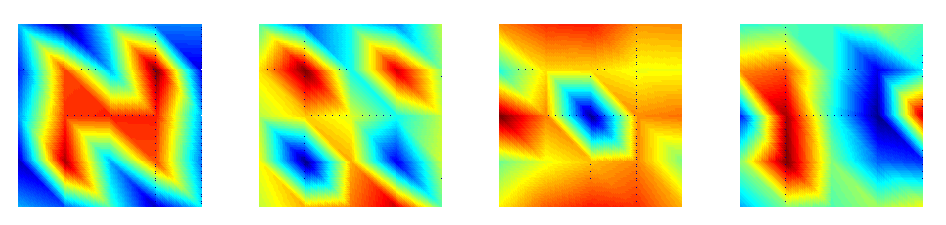
\includegraphics[width=0.5\textwidth]{fig11.eps}
  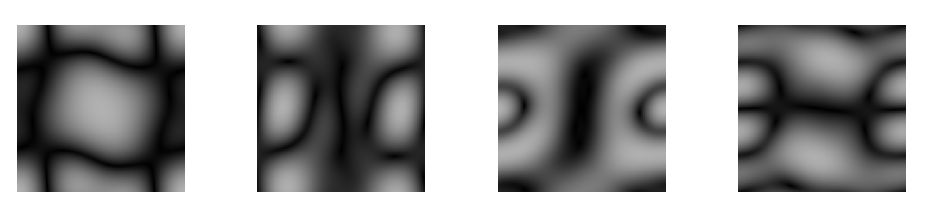
\includegraphics[width=0.5\textwidth]{fig12.eps}
    \caption{An example of learned filters and their Fourier spectrum.}
    \label{fig:1}
\end{figure}

So far, the models are based on the premise that the signals can be written exactly as a sparse linear combination of translational invariant wavelets. In practical applications, there may be perturbations or noises added to the coefficients, it is better to consider the following variant of model \eqref{model:m1} which allows small perturbations of the coefficients.
\begin{equation}
\label{model:m3}
\begin{aligned}
	&\min_{a_1,\cdots,a_m,v_1,\cdots,v_m} \sum_{i=1}^m \|v_i\|_1  + \lambda \sum_{i=1}^m \|v_i - a_i(-\cdot)*x\|_2^2\\
	\textrm{subject to} \quad& \{a_i\}_{i=1}^m \in \mathcal{C_\delta} \\		 
\end{aligned}
\end{equation}

We solve this optimization program using the split Bregman method\cite{goldstein2009split}. Details are given in the appendix.


A key feature of this variant  is that unlike the previous model, the wavelet coefficients $\{v_i\}$ is no longer linearly dependent on $x$ given the filters $\{a_i\}_{i=1}^m$. Yet the coefficients can still be computed efficiently. Indeed, given the learned filters $\{a_i\}_{i=1}^m$ and the new input signal $x$, the coefficients are obtained by 
\[
\min_{v_1,\cdots,v_m} \sum_{i=1}^m \|v_i\|_1 + \lambda \sum_{i=1}^m \|v_i - a_i(-\cdot)*x\|_2^2,
\]
the solution of which is given explicitly:
\[
v_i = \mathcal{T}_{1/2\lambda}( a_i(-\cdot)*x),\quad i=1,\cdots,m
\]
where $\mathcal{T}: \mathbb{R}\mapsto \mathbb{R}$ is the soft-thresholding operator defined by
\begin{equation}
\label{eq:soft}
\mathcal{T}_a(x)=\left\{ \begin{array}{lr}  (|x|-a)sign(x), &\textrm{ if } |x| > a \\0, &\textrm{otherwise}\end{array}\right . .
\end{equation}

When $\mathcal{T}$ operates on a vector, it operates on each component of the vector.


A special case of this variant, when the support of $a_i$ is of size $r\times r$ and $m=r^2$ and the filters are orthogonal to each other is proposed independently in \cite{cai2014data}. A local solution is found in an elegant manner by iteratively solving the $\{v_i\}_{i=1}^m$ and $\{a_i\}_{i=1}^m$.

To this end, we have introduced the construction of adaptive wavelet tight frames for one layer. When plugged into low level image processing applications, the results produced are comparable to those obtained by the dictionary learning paradigm, some numerical illustrations are given in section 5. In addition, we observed a quite unexpected and intriguing phenomena that we would like to share with the readers.

\subsection{An Intriguing Phenomenon}
\textbf{A unique low pass filter}. The most commonly used wavelets and wavelet tight frames constructed using MRA has only one low pass filter by design. As a result, it enables a fast multi-level decomposition and reconstruction algorithms, to get a multi-level representation of the signal, we successively apply the same filters to the coefficients representing the low pass information. This structure is illustrated in Figure \ref{fig:arch}a. The root node represents the input signal, the child nodes represent the coefficients, the leftmost node always represent the low frequency coefficients. On the other hand, as one can notice, the UEP does not distinguish between low pass and high pass filters, all the filters jointly satisfy an algebraic constraint. From this perspective, indeed, one can use multiple low pass filters at the cost of increased computational time. This is represented by multiple branching point in the tree diagram. For the algorithm to be of practical use, especially when computational efficiency is a concern, it is better to maintain a unique low pass filter. Taking this into consideration, one is attempted to add the following linear constraints to the previous model:
\begin{equation}
\label{eq:low}
\sum_{i\in\mathbb{Z}^2} a_1(i)=1,\quad \sum_{i\in \mathbb{Z}^2} a_k(i)=0, k\in\{2,\cdots,m\}
\end{equation}
If the above constraints are not incorporated, one would expect the resulting filters would be of diverse frequencies.

Surprisingly, we found that, on many datasets, the filters learned contains exactly one low pass filter even though the above constraints are not present. That is, constraint \eqref{eq:low} is automatically satisfied!  Numerically, we observed that for filter coefficients that are normalized to have unit $l_2$ norm, $ |\sum_{i\in \mathbb{Z}^2} a_k(i)| < 10^{-4}, k\in\{2,\cdots,m\}$. This phenomenon is relatively stable as we vary the number and support size of the filters. We observed this phenomenon on many datasets, including the "Extended Yale Face Dataset B"\cite{GeBeKr01}, the Caltech 101 dataset\cite{fei2007learning}, and a large number of randomly chosen natural photos. However, this phenomenon is not entirely universal, we observed multiple low pass filters on the MNIST dataset\cite{lecun1998gradient}. 

This phenomenon is reassuring in that the filters produced by \eqref{model:m1} now has exactly the same form as the familiar wavelets and wavelet tight frames, hence can be used in the precisely same way.

On the other hand, that fact that this phenomenon is ubiquitous in natural photos but not in images like MNIST tells us some partial information about the structure of the space of all "natural images", which traditional wavelets are known to compress very well. In hindsight, the coincidence that manually designed wavelets happen to agree with the adaptively learned filters with sparsity in mind partially explains the successful of JPEG2000 on compressing natural images.

From a practical point of view, one can always first try to solve \eqref{model:m1} without the low frequency constraint, and see if there happen to be a unique low frequency filter, if so, then there is a good chance that one can replace the wavelets or wavelet tight frames with adaptive versions at no additional cost. If not, one may consider incorporating the constraint explicitly.

\subsection{Recover Predefined Wavelets}
As the proposed model can be seen an adaptive version of the wavelet tight frame, it is therefore natural to ask when could we recover the wavelet filters. We did a numerical experiment to check this. We generate signal using linear combination of predefined wavelets of varied sparsity level of coefficients.  Then check whether the learned filters automatically recover the predefined wavelet filters. This question is related to the exact recover problem in dictionary learning. There, the problem is that suppose the data matrix $X$ is generated by linear combination of dictionary atoms $X=DC+\epsilon$, then ask under what conditions can we recover $D$ and $C$ simultaneously given the observations $X$? It can be shown that under some restrictive conditions, with high probability, we can achieve exact recovery, see \cite{spielman2013exact,arora2013new} for two recent results in direction. However, in our case, the dictionary is of special form and cannot be explained by the results there.

In the numerical experiment, we generate the signals of Daubechies wavelets with different level of sparsity and learn the filters by solving \eqref{model:m0}. Criterion of success is that the $l_2$ norm of the difference between the learned filters and the predefined filters is smaller than $10^{-4}$ ), we repeat each setting multiple times and record the ratio of success in the following table:
\begin{table}

\centering
\begin{tabular}{| c | c | c | c| c | c |}

\hline
Density & db2\_32 & db2\_64 & db3\_64 & db12\_64 & db24\_64 \\
\hline
0.1 & 1 & 1 & 1 & 1 & 1 \\
\hline
0.2 & 1 & 1& 1 & 1 & 1 \\
\hline 
0.3 & 1 & 1 & 1 & 1 & 1  \\
\hline
0.4 & 1 & 1 & 1 & 0 & 0  \\
\hline 
0.5 & 0 & 0 & 0 & 0 & 0 \\
\hline

\end{tabular}
\caption{Ratio of successful recovery of predefined wavelets.}
\end{table}
We note that if the signals indeed have a sparse representation in the wavelet domain, then the algorithm can successfully recover the wavelet filter. Above some threshold, however, the algorithm fails to recover the wavelet filters catastrophically. This is not surprising, after all the signals are no longer sparse in the wavelet domain. It's interesting to that there seems to be a phase transition between the success and failure regimes.


\section{Extension to Multiple Layers}
\subsection{Three Structures}
Now, we extend the previous construction of adaptive wavelet tight frames to multiple layers. Going from one layer to multiple layers, we consider three typical structures illustrated in Figure \ref{fig:arch}.
\begin{figure}[h!]
\begin{tabular}{l l l}
\subfloat[][]{
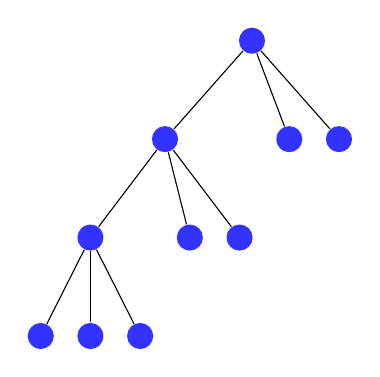
\begin{tikzpicture}[every tree node/.style={circle,fill=blue!80},
level distance=1.25cm,sibling distance=.3cm, 
edge from parent path={(\tikzparentnode) -- (\tikzchildnode)}]
\Tree [.\node {}; 
[.\node{};
[.\node{};
[.\node{};][.\node{};][.\node{};]][.\node{};][.\node{};]
]
[.\node{};
] 
[.\node{};
]]
\end{tikzpicture}
}
&
\subfloat[][]{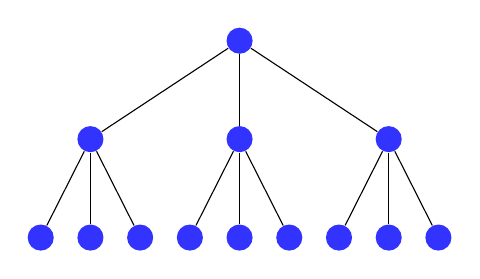
\begin{tikzpicture}[every tree node/.style={circle,fill=blue!80,align=center,anchor=center},
level distance=1.25cm,sibling distance=.3cm, 
edge from parent path={(\tikzparentnode) -- (\tikzchildnode)}]
\Tree [.\node {}; 
[.\node{};
[.\node(A){};][.\node{};][.\node{};]
]
[.\node(B){};
[.\node{};][.\node{};][.\node{};]
] 
[.\node{};
[.\node{};][.\node{};][.\node{};]
]]
\end{tikzpicture}
}
&
\subfloat[][]{
  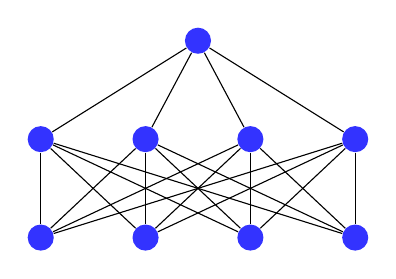
\begin{tikzpicture}[every tree node/.style={circle,fill=blue!80,align=center,anchor=center},
level distance=1.25cm,sibling distance=1cm, 
edge from parent path={(\tikzparentnode) -- (\tikzchildnode)}]
\Tree [.\node {}; 
[.\node(A1){};
[.\node(A2){};]
]
[.\node(B1){};
[.\node(B2){};]
] 
[.\node(C1){};
[.\node(C2){};]
] 
[.\node(D1){};
[.\node(D2){};]
]]
\draw (A1)--(B2);
\draw (A1)--(C2);
\draw (A1)--(D2);
\draw (B1)--(A2);
\draw (B1)--(C2);
\draw (B1)--(D2);
\draw (C1)--(A2);
\draw (C1)--(B2);
\draw (C1)--(D2);
\draw (D1)--(A2);
\draw (D1)--(B2);
\draw (D1)--(C2);

\end{tikzpicture}
}
\end{tabular}
\caption{three structures}





\label{fig:arch}
\end{figure}


The first structure is a $m$-ary tree which has at most one brunching point at each level. This corresponds to the multi-level fast wavelet or wavelet tight frame transform. The root node represents the input image, the nodes represents the coefficients, the leftmost node always represents the low frequency coefficients.(for illustration purpose, the input image has only one channel), applying $m$ filters on the input, we get $m$ sets of wavelet tight frame coefficients. Each set of coefficients is represented using $m$ child nodes. The left most node always represents the low frequency coefficients. To do multi-level transform, we successively apply the same filters on the low frequency coefficients. Thus, the structure corresponding to a level $L$ wavelet tight frame transform is a tree of depth $L+1$ . 

This structure arises naturally in wavelet tight frames generated using MRA. The major advantage are the efficient decomposition and reconstruction algorithm. For level-$L$ transform with downsampling, it takes only $\mathcal O(mN)$ operations for the decomposition of a signal of length $N$. To apply structure, the existence of a single low pass filter is assumed. We can extend the previous one layer construction to this structure if there happen to be one low pass filter or is constrained to have only one low pass filter.  This structure is mostly useful in image compression tasks, and the coefficients are critically down-sampled.

The second structure is a full $m$-ary tree. Compared with the first architecture, instead of doing transforms on the low pass coefficients only,  transforms are performed on all the coefficients.  Apparently, the computational cost is now much larger. It is not appropriate for image compression tasks, but it is good for classification. An incarnation of this structure for classification is the scattering transform\cite{bruna2013invariant}. Adaptation of the one layer model to this structure is straight forward. As the computational cost grows exponentially with the number of layers, we have to implement this structure with care, and use some pruning procedures, for example, we can stop expanding the node if it has very small energy.

The third structure resembles that of a convolutional neural networks. The first layer is still the same as the previous two, below that, the tree structure is replaced by a  locally connected  convolutional structure. This structure is more elaborate and requires some explanation which we give in the next subsection.

\subsection{The Multi-scale Structure}
The architecture consists an input layer and a few intermediate layers. The first layer is the same as the previous two structures. The intermediate layer accepts as input a few sets of coefficients produced by the previous layer, and produces another sets of output coefficients, not necessarily of the same size. The input and output can be thought of as multi-channel images. The goal of the layer is still to produce sparse approximations of the input. Let $\{x_1,\cdots,x_m\}$ be the input coefficients, $\{v_1,\cdots,v_n\}$ be the output coefficients. The decomposition for the noise free case is defined as:
\begin{equation}
v_j = \sum_i a_{ij}(-\cdot)*x_i,\quad j=1,\cdots,n
\end{equation}
and the reconstruction is defined as 
\begin{equation}
x_i = \sum_j a_{ij}*v_j, \quad i=1,\cdots, m.
\end{equation}
The objective is to learn $\{a_{ij}\}_{i\leq m,j\leq n}$ which gives the sparest representation within the class of perfection reconstruction filters. Recognizing this as a 3D convolution, the UEP condition without downsampling then reads:
\begin{equation}
\label{uep:3d}
\sum_{i=1}^m\sum_{j=1}^n  \sum_{n\in \mathbb{Z}^3} a_{ij}(k+n)a_{ij}(n) = \delta(k).
\end{equation}

We could explicitly incorporate this constraint and repeat what did in the previous sections. This amounts to solving
\begin{equation}
\begin{aligned}
	&\min_{ \{a_{ij}\} } \sum_j \|v_j\|_1 \\
	\textrm{subject to} &\quad v_j = \sum_i a_{ij}(-\cdot)*x_i \\
		&\{a_{ij}\} \textrm{ satisfies \eqref{uep:3d}} \\
\end{aligned}
\end{equation}
On the other hand, we could solve a sampled approximation of the UEP constraint as
\begin{equation}
\label{eq:m3}
\begin{aligned}
\min_{a_1,\cdots,a_m, v_1,\cdots,v_m}& \sum_j \|v_j\|_1 \\
 \textrm{s.t.}  \quad &v_j = \sum_{i} a_{ij}(-\cdot)*x_i \\
	&u_j=\uparrow\downarrow(\sum_i a_{ij}(-\cdot)*y_i), \forall j. \\
	&\sum_i \|y_i - \sum_j a_{ij}*u_j\|_2 \leq \delta 
\end{aligned}
\end{equation}

where $y$ is randomly sampled vectors of sufficient size, and the $\uparrow \downarrow$ represented a down-sampling followed by a up-sampling operation. It could be omitted if we are only interested in un-decimated wavelet tight frames. The sampling operator need not be linear, it could be, for example max pooling and it reverse which are defined as 
\[
\downarrow(c_1,\cdots,c_n) = (\arg\max_{c_1,\cdots,c_n} |c_i|, \arg\max_{i=1,\cdots,n} |c_i|)
\]
and its reverse
\[
\uparrow(v,p)=(0,0,v[p],\cdots,0) \textrm{ with $v$ at the $p$-th location}.
\]
This is particularly useful for classification tasks.Unlike the linear sampling, in this case, we have to record both the value and position to get a natural reverse operation.

Similar to what we did before, we consider the following variant which we use in the numerical experiments.
\begin{equation}
\label{eq:m5}
\begin{aligned}
\min_{\{a_{ij}\}, v_1,\cdots,v_m}& \sum_j \|v_j\|_1 + \lambda \sum_j \|v_j-  \sum_{i} a_{ij}(-\cdot)*x_i \|_2^2\\
 \textrm{s.t.}  	\quad 	u_j&=\uparrow\downarrow(\sum_i a_{ij}(-\cdot)*y_i), \forall j.\\
&\sum_i \|y_i - \sum_j a_{ij}*u_j\|_2  \leq \delta\\
\end{aligned}
\end{equation}
There is a subtlety considering stacking intermediate layer to form a multi-scale structures. That is, the output to input relation cannot be linear, otherwise the multiple layers would just contracts to one layer. The non-linearity in our model may come from two sources: one is the nonlinear sampling procedure, the other is the thresholding in the encoding stage.

Using \eqref{eq:m5} as a building block, we stack multiple layers together, we finally get the multi-scale structure depicted in Figure \ref{fig:arch}c. The filters are learned in a  layer by layer fashion, starting with the first one. Once the optimization has converged for the layer, we then move on to learn the next while keeping all filters in previous layers fixed. 

\section{Numerical Illustrations}
The models discussed so far is merely a view point. The only way to tell if these models work in reality is to apply them. In this section, we provide examples to illustrate the effectiveness of the proposed representation. Examples in image compression, denoising, classification will be given. This section is meant for illustration purpose only ans is by no means an exhaustive comparison of different methods.
\subsection{Image Compression}
Compression using adaptive wavelet tight frames that induces sparsity seems to be a very natural approach. Nevertheless, developing a mature compression scheme that competes favorably with JPEG2000 is very hard, as in JPEG2000 the entropy coding stage has been perfected. It is not sufficient to provide only the representation stage, one must provide appealing entropy coding as well. Still, we can address a specific coding task, where the entropy coding stage becomes secondary. 

When we consider a narrow and specific class of images, the amount of redundancy increases, hence enabling a better compression performance. In particular, we can use a single image. We compare two elementary compression schemes, one is predefined wavelet tight frames generated from Daubechies wavelets, db3, the other is the adaptive wavelet tight frame, which has $4$ filters of size $6\times 6$ and is trained on the clean image \ref{fig:bar}(a).  The adaptive wavelet tight frame and the predefined wavelet tight frame has the same support size and the same total number of filters.  Given a tight frame and an image, we perform a 7-level transform, and keep only a fixed fraction of the coefficients with largest absolute values. The proportion of kept coefficients ranges from $1/2$ to $1/20$. Those coefficients are then used to reconstruct the image. We use PSNR(peak signal to noise ratio) to measure the quality of the compressed image. The result is shown in Figure \ref{fig:3}
\begin{figure}[h!]
    \centering
    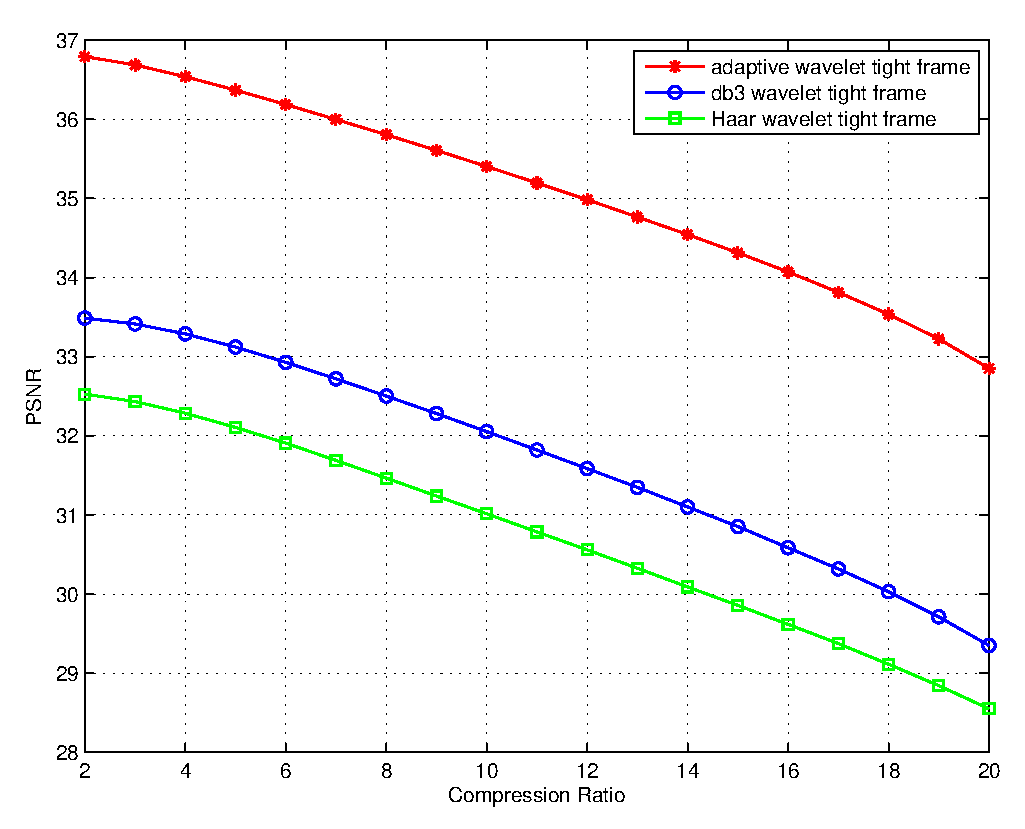
\includegraphics[width=0.4\textwidth]{figure51.eps}
    \caption{image compression illustration}
    \label{fig:3}
\end{figure}
The adaptively constructed tight frames is shown to be more effective.
\subsection{Image Denoising}
Images often contain noise, which may due to sensor imperfection, pool illumination, etc. Removing such noise is of benefit in many applications. Being perhaps the simplest possible inverse problem, it provides a convenient platform over which image processing ideas and techniques can be tested. Numerous contributions in the past few decades address this problem from many diverse point of view. The simplest of which is perhaps the wavelet domain thresholding. Later more sophisticated methods were developed and showed better performance such as the nonlocal means\cite{buades2005non}, BM3D\cite{dabov2007image}, and the more recent ones based on dictionary learning ideas\cite{elad2006image}. 

We have no intention of providing a survey of this vast activity on image denoising in this subsection. Instead, for the same illustration purpose, we demonstrate the results of applying adaptive wavelet tight frames to this problem and compare it with a specific model of interest, the K-SVD model\cite{elad2006image}. As it is closely related to the proposed model and is shown to achieve state of the art results.

We assume the image is corrupted by some additive noise. That is 
\[
g=f+n
\]
where $f$ is the clean image, $g$ is our observation, and $n$ is the noise with unknown distribution.The algorithm using adaptive wavelet tight frames is similar to wavelet domain thresholding: let $W$ be the decomposition operator associated with the wavelet tight frame, given a noisy image $g$, choose a scalar $\lambda$, then the denoised image is
\[
\hat{g} :=W^T \mathcal{T}_{\lambda} (Wg)
\]
where $\mathcal{T}$ is the soft thresholding operator introduced in \eqref{eq:soft}. $\lambda$ obviously depends on the noise level, choice of $\lambda$ requires some prior knowledge. Unlike image compression, in image denoising applications, we can afford using very redundant systems. The extra redundancy is proven to yield better results than the critically sampled wavelet frames. Therefore, we use relatively redundant systems in the three examples below.

In this first example, the input is single image normalized to $[0,1]$ and is corrupted with additive gaussian noise with $\sigma=0.1$. We train the filters both from the noisy image and clean image. The filter is of support size $6\times 6$ and we train $36$ of them .The result is in Figure \ref{fig:bar}.  The PSNR shown is selected by grid search to produce best PSNR. It is not surprising that the filters learned from a clean image produces better quality image. The performance of K-SVD algorithms depends on the number of the atoms in the dictionary. Generally, the performance increases as we increase the number of atoms as long as the number is not too large. In this example, $256$ atoms with size $6\times 6$ is used.

\begin{figure}[h!]
\centering
\label{fig:bar}
\begin{tabular}{c c c c}
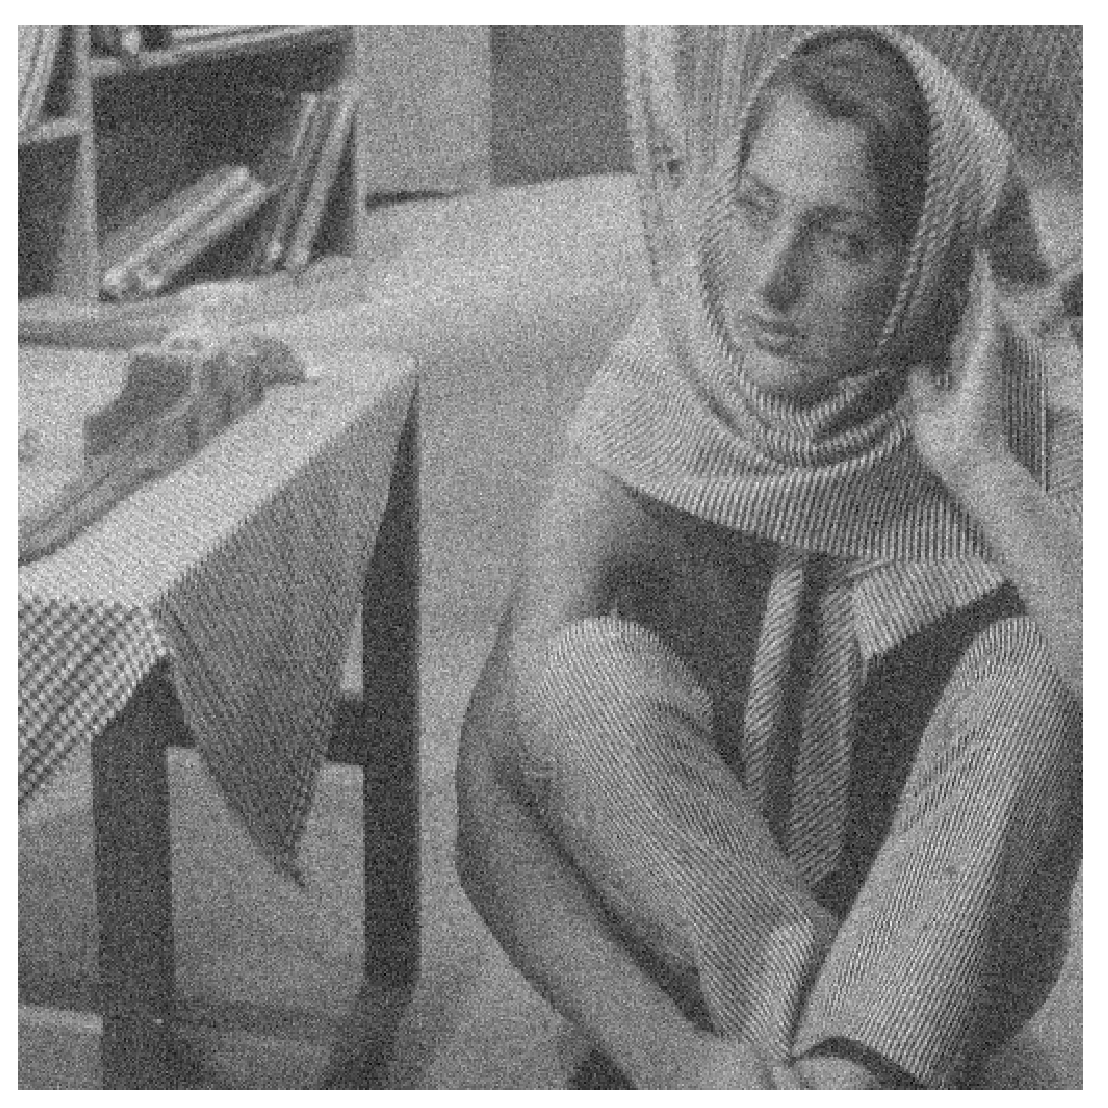
\includegraphics[width=3cm]{./figures/4_1_noise.eps} & 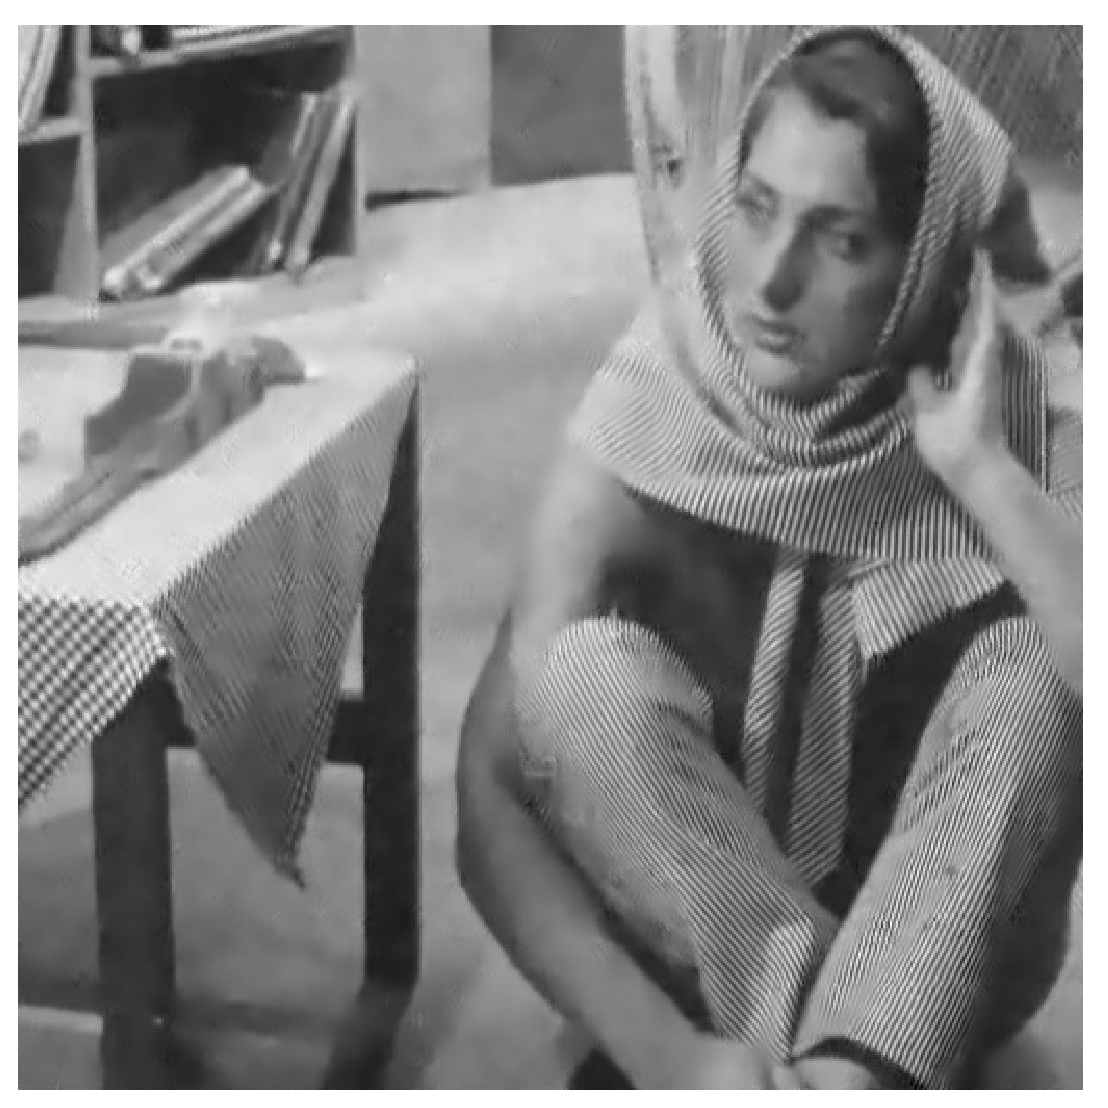
\includegraphics[width=3cm]{./figures/4_3_ksvd.eps}
&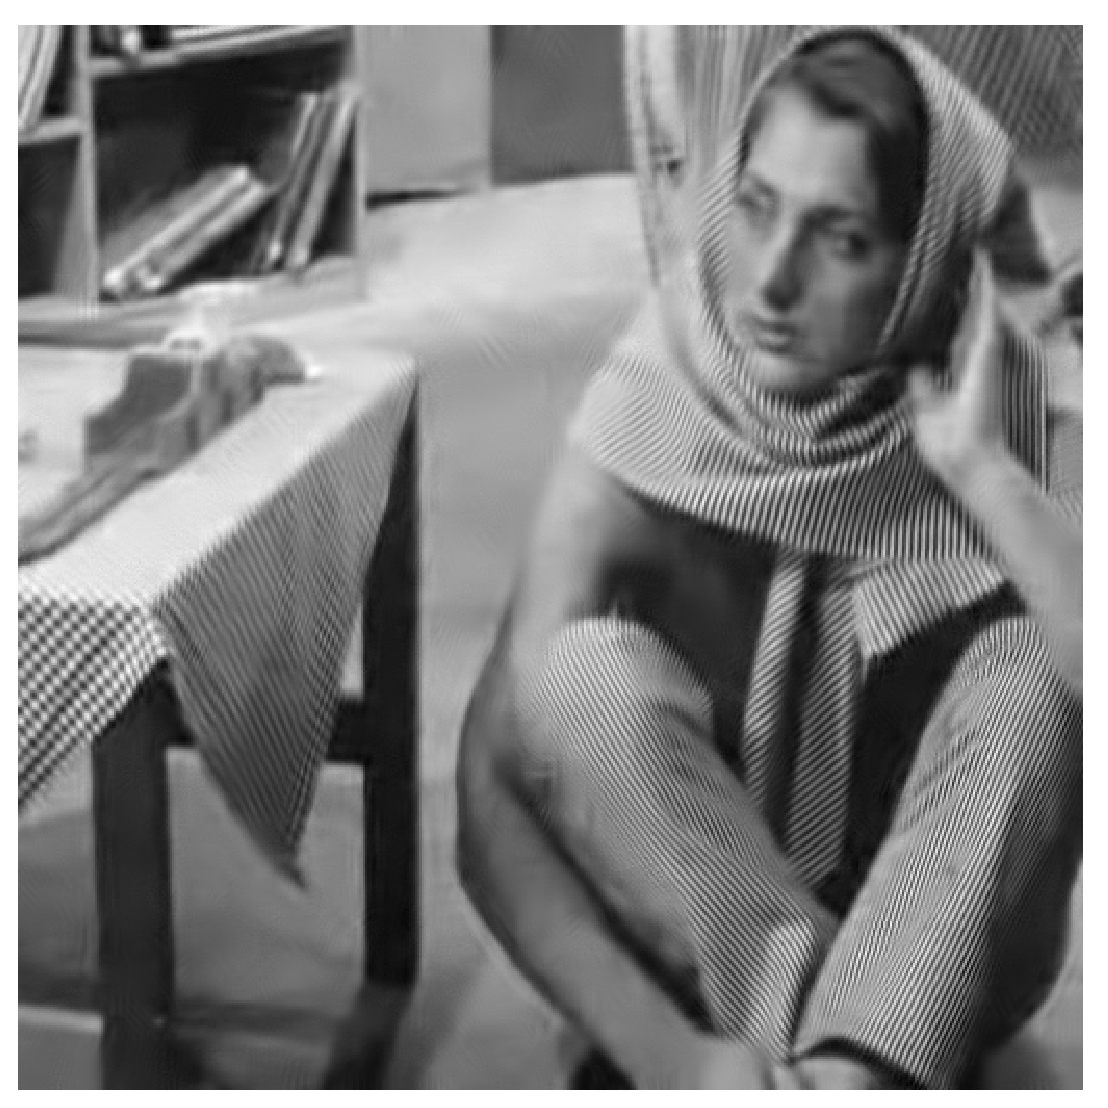
\includegraphics[width=3cm]{./figures/4_4_tfnoise.eps} & 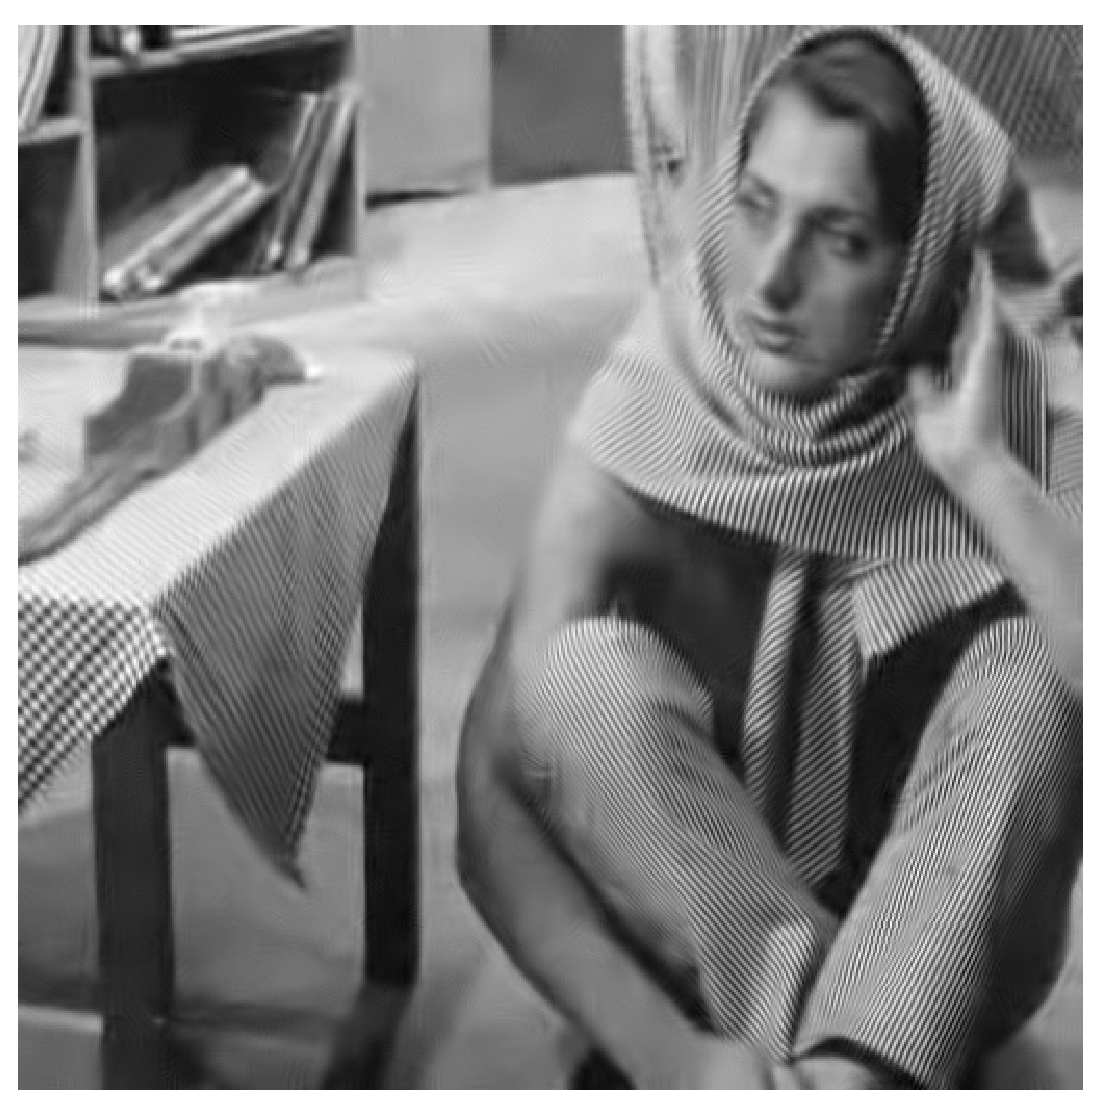
\includegraphics[width=3cm]{./figures/4_5_tfclean.eps}\\
 (a)noisy image ($\sigma=0.1$)& (b)K-SVD(28.65dB) &(c)model \eqref{model:m0}(28.8dB) & (d)model \eqref{model:m0}(29.3dB) 
\end{tabular}
\caption{results of denoising. (b)(c) are trained on the noisy image, (d) is trained on the clean image.}
\end{figure}
The adaptive wavelet tight frames trained from clean is able to recover fine textures of the image, as shown in Figure \ref{fig:detail}.
\begin{figure}[h!]
\centering
\label{fig:detail}
\begin{tabular}{c c c}
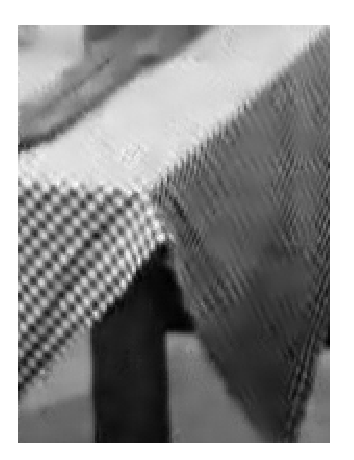
\includegraphics[width=3cm]{./figures/4_7.eps} & 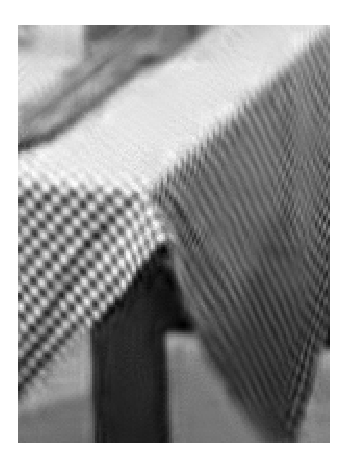
\includegraphics[width=3cm]{./figures/4_8.eps} &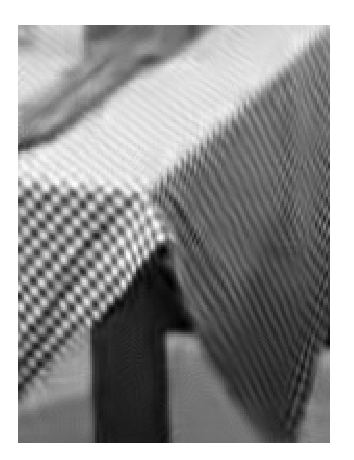
\includegraphics[width=3cm]{./figures/4_6.eps}\\
K-SVD & model \eqref{model:m0} & model \eqref{model:m0} \\
(a)&(b)&(c)\\
\end{tabular}
\caption{(a)(b) are trained on the noisy image, (c) is trained on the clean image.}
\end{figure}
There is a natural scenario where training filters from clean images makes sense.Imagine the dataset of human face images, some of them are corrupted by noise. We would like to train the filters from the clean images and apply them to the noisy images. We test this idea on the extended Yale human face dataset B. A glimpse of the dataset is in Figure \ref{fig:yale}. We also add additive gaussian noise with $\sigma=0.1$. 
\begin{table}[h!]
\centering
\begin{tabular}{c c c c}
\hline
& K-SVD & model \eqref{model:m0} noisy& model \eqref{model:m0} clean \\
\hline
PSNR& 31.4dB &31.35dB& 32.07dB\\
\hline
\end{tabular}
\caption{model \eqref{model:m0} noisy is learned on noisy images, model \eqref{model:m0} clean is learned on clean images.}
\end{table}

\begin{figure}
\centering
\label{fig:yale}
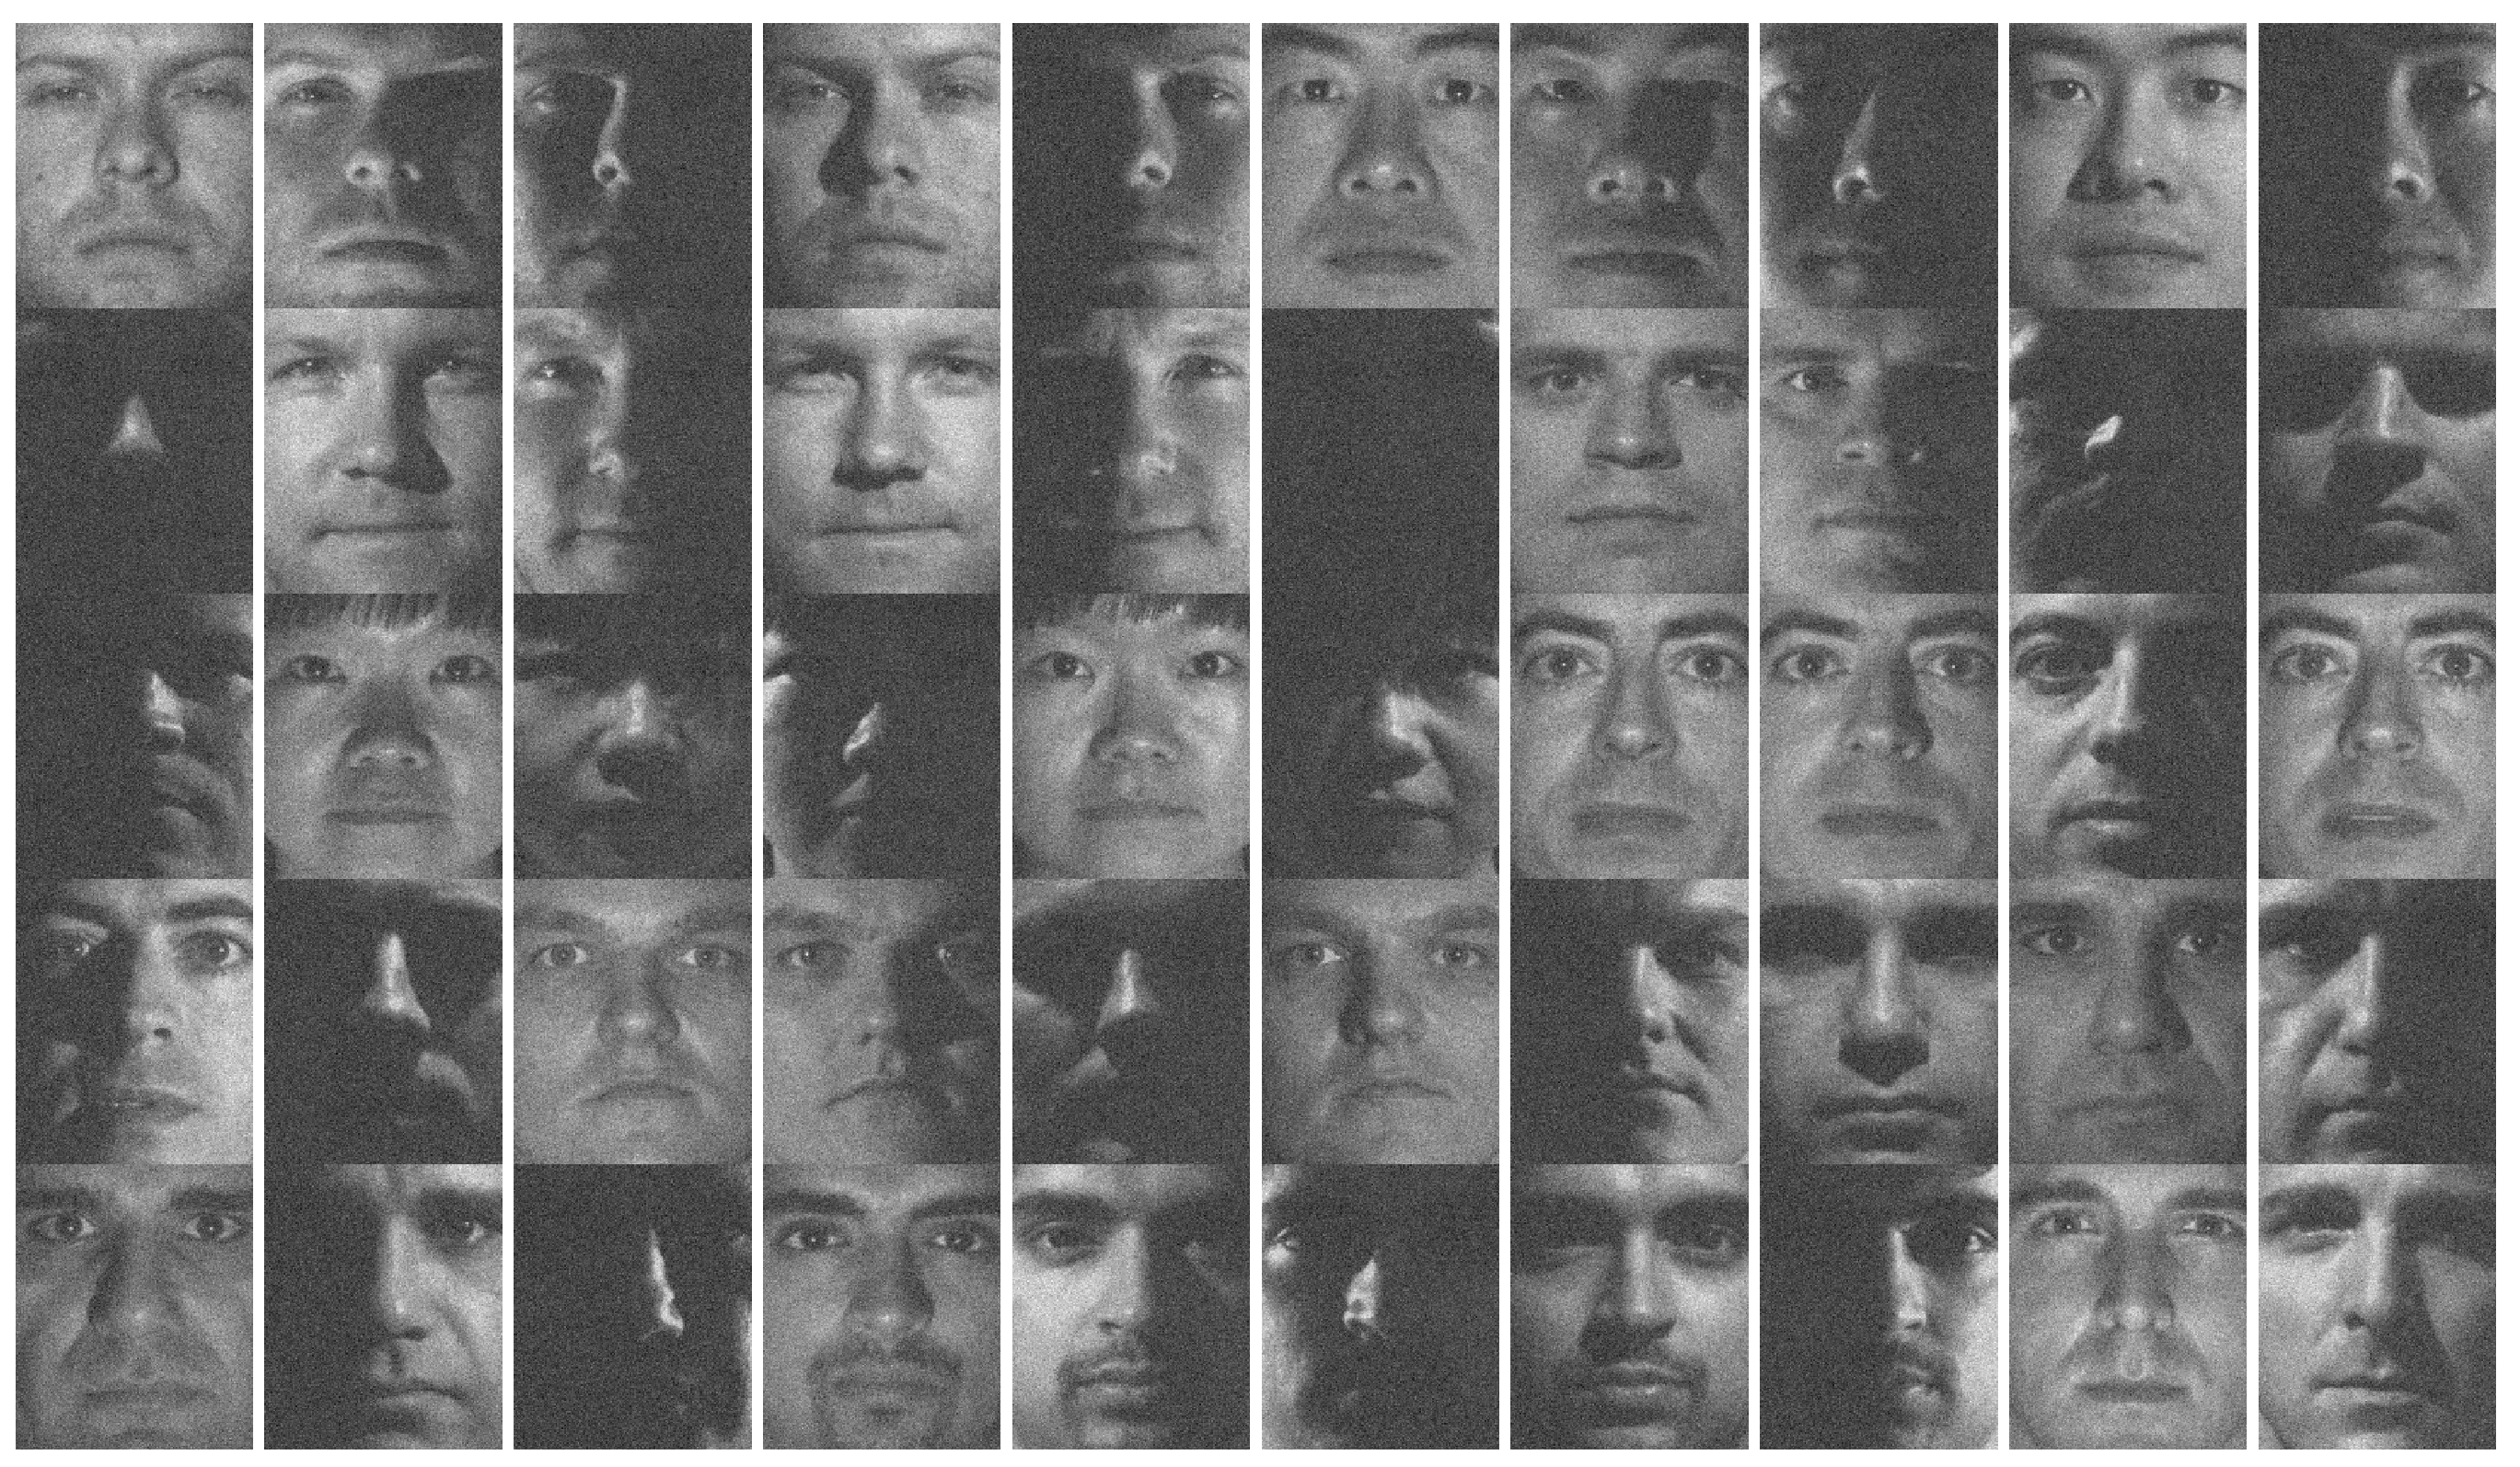
\includegraphics[width=6cm]{./figures/3_2.eps}
\caption{noisy images of extended Yale face dataset B}
\end{figure}
The third example is natural images with unknown noise. The two images are collected form the Internet. Same as the previous two examples, we learn filters directly from the image. As the image has 3 channels, we learn the filters on each channel separately. $\lambda$ is the same on three channels and is chosen to yield good visual. 

\begin{figure}[h!]
\centering
\begin{tabular}{c c}
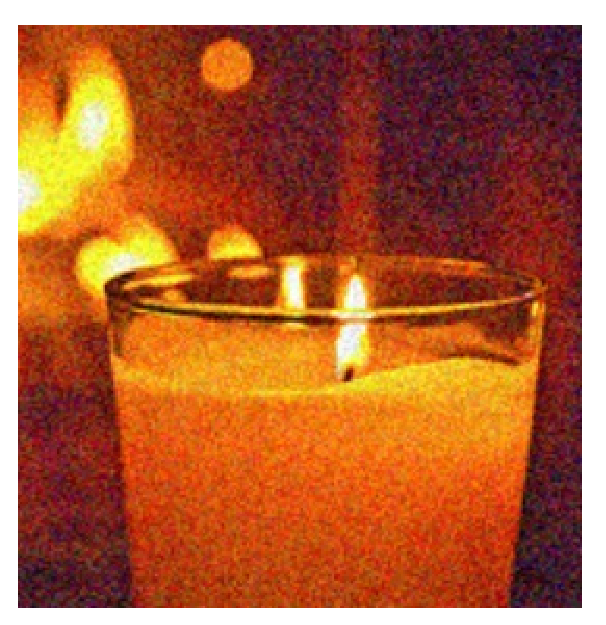
\includegraphics[width=4cm]{./figures/candle_noise.eps} & 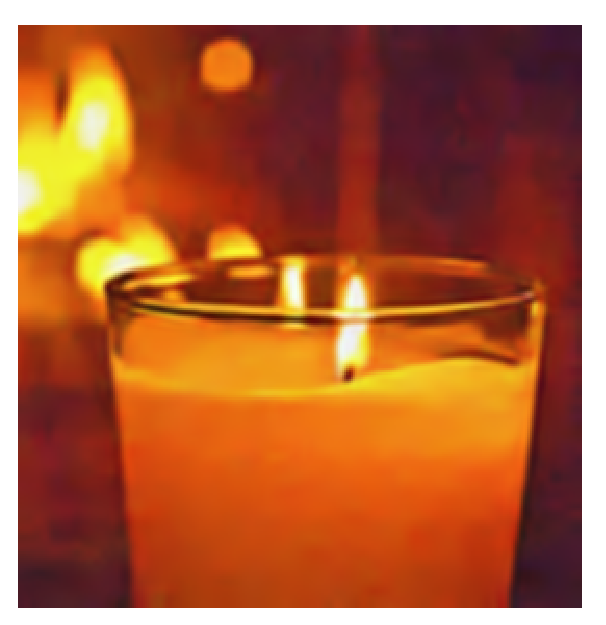
\includegraphics[width=4cm]{./figures/candle_clean.eps}\\
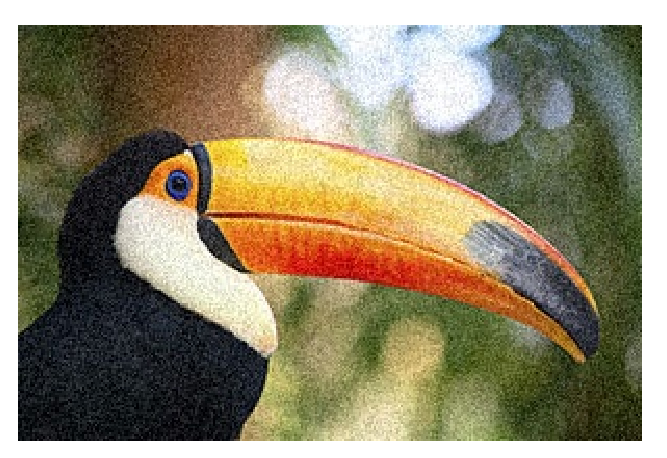
\includegraphics[width=4cm]{./figures/bird_noise.eps} & 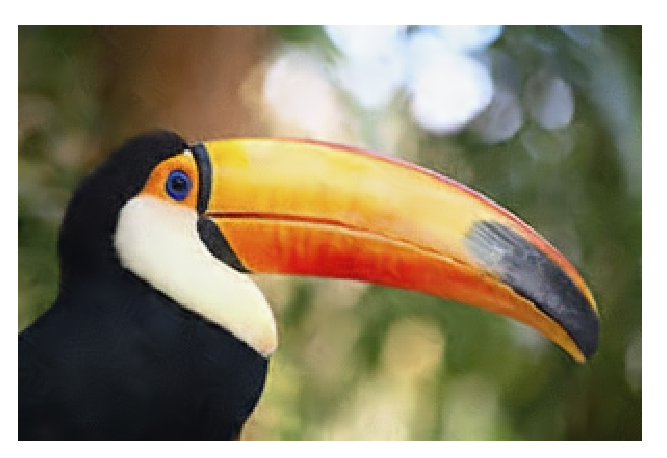
\includegraphics[width=4cm]{./figures/bird_clean.eps}\\
\end{tabular}
\caption{denoising example of two color images}
\end{figure}

\subsection{Classification}
The proposed model is aimed to produce sparse representations, it happens that sometimes sparse representations help classification tasks. In this experiment, we apply the representation obtained using the proposed model to examine its effectiveness on classification tasks. We choose to test on the MNIST handwritten digits dataset. It contains 70000 $28\times 28$ images of digits from 0 to 9, 60000 for training and 10000 for testing. We adopt the second and third structure with two layers. Rectified linear activations are applied after the first layer. To do classification, we then send the output coefficients to a linear SVM.  Results with different number of filters are summarized in the following table.
\begin{table}[h!]
\centering
\begin{tabular}{c c c c c}
\hline
MNIST & Raw pixel & $6$ filters $6\times 6$ & $12$ filters $6\times 6$& 2 layers \\
\hline
Precision & 94.2\% & 97.0 \% & 97.4\% & 99.0\% \\
\hline
\end{tabular}
\caption{MNIST classification}
\end{table}
There is a significant reduction in the error rates compared to raw pixel features. The proposed models are worse than state-of-the-art results which are obtained using convolutional neural networks and virtual SVM, the best reported result without expanding the training set is 0.53\%, nevertheless, this experiments demonstrates the proposed models provide a redundant and sparse representation of the signal that is more linearly separable than the original one.

\section{Discussions}
\subsection{Compare Dictionary Learning and the Proposed One Layer Model}
As we will see in this section, the dictionary learning models and model A share some similarities and have some differences. We make the following remarks: 

\textbf{1. Model \eqref{model:m0} is convolutional form of dictionary learning in the small $\lambda$ regime, with constraints}. Consider the training procedure of dictionary learning, given an image or a set of images, we collect all $r\times r$ non-overlapping patches and form them into a data matrix $X$, then we solve the following minimization program:
\begin{equation}
\min_{D,C} \|X-DC\|_2^2 + \lambda\|C\|_1.
\end{equation}
The underlying rationale is at some scale, say $r$, the image patch can be approximated by a sparse combination of some basis vector, where each column of $D$ represents a base vector and each column of $C$ represents the combination coefficients for a particular patch.
Consider the proposed model \eqref{model:m0}. With some reorganization, this can be brought into a form that is very similar to dictionary learning. Let $X$ be the matrix formed by collecting all overlapping $r\times r$ images from an image, where each column of $X$ represents a vectorized image patch. Let $A=(vec(a_1),\cdots, vec(a_m))$, and $V$ is coefficient matrix which is reshaped conformally. Then \eqref{model:m0} is equivalent to the following model in the small $\lambda$ region.
\begin{equation}
\begin{aligned}
&\min_{A,V} \|X-AV\|_2^2+\lambda \|V\|_1. \\
&\textrm{subject to}\quad V=W_a X
\end{aligned}
\end{equation}
The objective is of the same form as in dictionary learning except for that in dictionary learning, the $X$ is formed from non-overlapping patches while in the proposed model,  $X$ is formed from overlapping patches. If we accept the premise that image patches are translation invariant at a certain small scale, then overlapping patches is a natural choice. In fact, for the purpose of finding optimal local basis, we could form $X$ aggressively by sampling randomly uniformly from the image. When the sample size is large, the resulted basis converges to the one obtained by solving \eqref{model:m0}. The way dictionary learning forms the matrix $X$ corresponds to uniform sampling from a special non-lapping grid, which is more or less unnatural. 

Besides the formal similarity, there is a  big difference in the constraint. The dictionary learning problem is unconstrained, as a result, the coefficients obtained by solving sparse coding are in general sparser, but the decay of the coefficients does not reflect the regularity of the signal being approximated. On the other hand, the coefficients obtained by the proposed model are normally less sparse, but the model takes into account the regularity of the signal and more importantly, is fast to compute. There are also some difference between the two models in practice. For example, In the practice of training dictionary learning models, people often use very large number of dictionary atoms(256 or more), whereas in convolutional bases, people only use a small number of basis function(usually no more than 32). The patch based reconstruction results visually unpleasant block effect, which needs to be removed by post processing, while the proposed model does not have such an issue.(But critically sampled model may suffer from block effect depending on the support of the filter.)

\textbf{2. The proposed model generalizes to multiple layers}. Being able to extend to multiple layers is crucial to a multi-scale representation. However, dictionary learning, in its original form, cannot achieve this objective. In dictionary learning, a dictionary is obtained and each image patch is associated with a few combination coefficients. As these coefficients are unordered and are of different length for different image patches, there is no obvious way how to continue learning the pattern of the coefficients in a similar "dictionary learning" fashion. In comparison, in the proposed one layer model, the coefficients associated with the image are still placed on a regular grid, which, after downsampling, are still of the same shape as the input, which facilitates further learning in almost the same way. It is this feature that allows the proposed one layer model to extend to multiple scales. 

\textbf{3. Computationally, the proposed model is favorable to dictionary learning}. When the parameters of both models are trained and to be used for inference, the computational costs are different. To infer the codes of a new incoming signal, dictionary learning performs a sparse coding, common procedures include matching pursuit and orthogonal matching pursuit\cite{tropp2007signal}, they are of high computational complexity as demonstrated in the introduction. In comparison, in the proposed model, only some convolutions plus a point-wise operation( such as thresholding) are performed. This is a dramatic performance gain.

\subsection{Connection with convolutional neural network}
The analysis based multi-scale structure resembles the deep convolutional neural networks even though we starts from a very different perspective. But this similarity are merely formal,there are some striking difference between them. First, the convolutional neural network is a supervised learning machine, while the proposed model is unsupervised. Second, the proposed model is constructed with respect to the unitary extension principle, hence has the nearly perfect reconstruction property, whereas in deep convolutional neural networks, it is not clear how to reconstruct the input as much information is lost as we ascend the layers along with operations like max pooling and rectified linear units. The proposed model is a nearly lossless decomposition of the input signal(as long as the number of filters in the intermediate layers are above a threshold), while the convolutional neural network is not. Studying the deeper connections between the analysis based multi-scale representations and the convolutional neural nets will be a future direction.

\section{Conclusion}
In this paper, we proposed a novel model that serves as a multi-scale adaptive representations of image signals. This representation improves over dictionary learning in two ways: first, encoding efficiency is dramatically improved, second, it is truly multi-scale. The proposed model also raises some interesting questions such as how to explain the unique low pass phenomenon? We hope that the proposed model can be an alternative to existing predefined wavelet tight frames and dictionary learning approach in some applications.
\section{Appendix}
\subsection{Numerical Algorithms}

The optimization program \eqref{model:m1} can be solved using interior-point method, but it is relatively slow  for large problems. We also consider the following split Bregman algorithm, which is faster. The program we want to solve is 
\begin{equation}
\begin{aligned}
&\min_{a_1,\cdots,a_m} \sum_j \|v_j\|_1 \\
\textrm{subject to} \quad & v_j = a_j(-\cdot)*x \\
	& \{a_i\}_{i=1}^m \in \mathcal{C}.
	\end{aligned}
\end{equation}

The split Bregman algorithm for this program can be written in the following steps:
\begin{equation}
\label{breg:all}
\begin{aligned}
	(v^{k+1},a^{k+1}) &=\arg\min_{v,a} \sum_j \|v_j\|_1 + \lambda\sum_j\|a_j(-\cdot)*x+b_j^k-v_j\|_2^2 \quad\textrm{subject to} \quad \{a_i\}_{i=1}^m \in \mathcal{C}.\\
	b_j^{k+1} &= b_j^k + a_j^{k+1}(-\cdot)*x - v_j^{k+1} \\
\end{aligned}
\end{equation}

The first step can be subdivided into two steps:
\begin{equation}
\label{bregv}
		v^{k+1}  = \arg\min_{v_1,\cdots,v_m}  \sum_j \|v_j\|_1 + \tau \|a^k_j(-\cdot)*x +b^k_j -v_j\|_2^2
\end{equation}
\begin{equation}
\label{brega}
a^{k+1} =\arg\min_a \sum_j \|a_j(-\cdot)*x+b^{k}_j-v^{k+1}_j\|_2^2   \quad\textrm{subject to} \quad \{a_i\}_{i=1}^m \in \mathcal{C}.\\
\end{equation}

Now \eqref{bregv} is given explicitly by soft thresholding:
\begin{equation}
	v^{k+1}_j = \mathcal{T}(a^k_j(-\cdot)*x+b^k_j,\frac{1}{2\lambda})
\end{equation}
and \eqref{brega} can be solved using interior point method. It makes no sense to solve $a$ beyond the precision of the uncertainty of $b$, a handful iterations will work. If the low frequency constraint is explicitly incorporated, the interior point steps should also be changed accordingly. Updating $b$ is straightforward.

Solving \eqref{eq:m3} basically follow the same lines, except that updating $a$ and $u$ is an unconstrained program hence we can run a few steps of conjugate gradient or quasi-Newton iterations to get desired accuracy.

Training for multi-layer case is achieved in a layer wise fashion. We first train the filters on the lower level(near the input), once they converge, the filters on the next level can be trained while keeping all the filters below fixed.








\bibliography{ref}
\bibliographystyle{plain}

\end{document}